\chapter{\heiti Product Description}
%\pagestyle{plain}
\pagenumbering{arabic}
\fancypagestyle{plain}
{
\fancyhf{}
\renewcommand{\headrulewidth}{2.4pt}
\renewcommand{\footrulewidth}{2.4pt}
\lhead{
    \setlength{\unitlength}{1mm}
    \begin{picture}(0,0)
    \put(0,0){\includegraphics[width=0.9cm]{logo.eps}}
    \end{picture}
    }
\chead{}
%\rhead{\xiaosi{合肥量子精密仪器有限公司}}
%\fancyfoot[LO,RE]{\xiaosi{ASG-GT50-C用户手册}}
\rhead{\sihao\textbf{Hefei Quantum Precision Devices Co., Ltd}}
\fancyfoot[LO,RE]{\sihao{ASG-GT50-C Manual}}
\cfoot{}
\fancyfoot[RO,LE]{\xiaosi\textbf{\thepage}}
}


\pagestyle{fancy}
\renewcommand{\headrulewidth}{1.5pt}
\renewcommand{\footrulewidth}{1.5pt}
\lhead{
    \setlength{\unitlength}{1mm}
    \begin{picture}(0,0)
    \put(0,0){\includegraphics[width=0.9cm]{logo.eps}}
    \end{picture}
    }
\chead{}
%\rhead{\xiaosi{合肥量子精密仪器有限公司}}
%\fancyfoot[LO,RE]{\xiaosi{ASG-GT50-C用户手册}}
\rhead{\sihao\textbf{Hefei Quantum Precision Device Co., Ltd}}
\fancyfoot[LO,RE]{\xiaosi{ASG-GT50-C Manual}}
\cfoot{}
\fancyfoot[RO,LE]{\xiaosi\textbf{\thepage}}

\setcounter{page}{1}
\setmainfont{Times New Roman}
\section{Inspect the Product Packaging}
\hspace{-0.2cm}When you received the product, if the package is damaged, keep the damaged packing container and cushioning material, then contact with us.
%用户收到产品后,请先检查包装是否完整,若包装已损坏,请保留被损坏的包装与防震材料,并及时与我司联系。

\section{\heiti Inspect the Accessories}
\hspace{-0.2cm}Please check the accessories according to the packing lists. If the accessories are incomplete or damaged, please contact with us.
%请根据装箱单检查随机箱附件,随机箱附件包括电源适配器一个,U盘一个,USB连接线一根。如有损坏或缺失,请及时与我司联系。

\section{\heiti Inspect the Instrument}
\hspace{-0.2cm}In case of any damage, or defect, or failure, please contact with us.
%如产品存在机械损坏,或者产品未通过性能测试,请您及时与我司联系。

\section{\heiti Appearance and Dimensions}
\hspace{-0.3cm}The appearance and dimensions of ASG-GT50-C are shown in Fig 1.1 (Front Panel), Fig 1.2 (Rear Panel), Fig 1.3 (Side Panel), and the unit is mm.
%ASG-GT50-C的外观与尺寸如图1.1(机箱前面板)、图1.2 (机箱后面板)、图1.3(机箱侧面板)所示,单位为mm。
\begin{figure}[ht]
\centering
%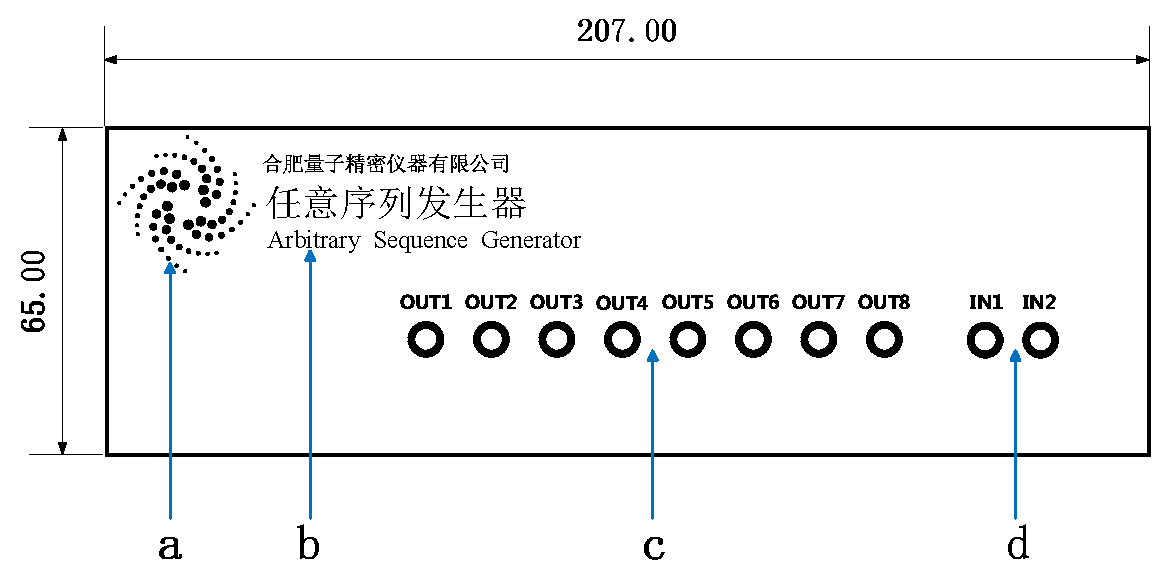
\includegraphics[width=14cm,height=6.5cm]{fig1_1}
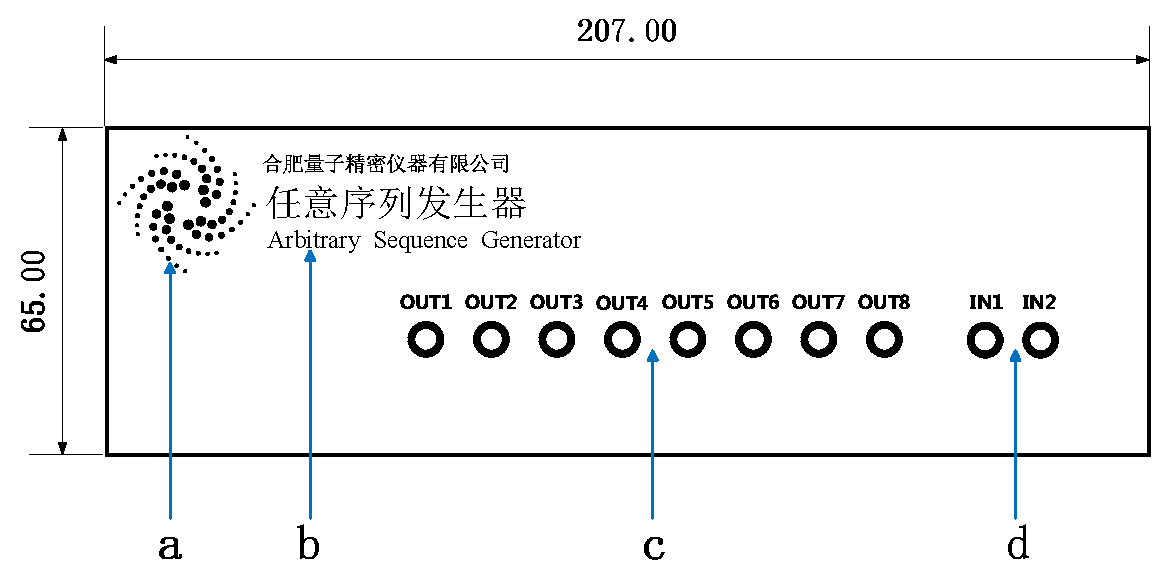
\includegraphics[height=6.5cm]{fig1_1}
\caption{\hspace{0.2cm}ASG-GT50-C Front Panel}\label{fig:fig1_1}
\end{figure}


\noindent \textbf{a.} The registered trademark of Hefei Quantum Precision Devices Co., Ltd\\
\textbf{b.} Name of the company and product \\
\textbf{c.} 8 output channels \\
\textbf{d.} Customized  input channels for user  

%\noindent \textbf{a.} 合肥量子精密仪器有限公司注册商标。\\
%\textbf{b.} 公司名称与产品名称。\\
%\textbf{c.} 共 8 个方波输出通道。\\
%\textbf{d.} 客户定制化功能通道。

%\newpage
\begin{figure}[ht]
\centering
%\includegraphics[width=14cm,height=6cm]{fig1_2}
\includegraphics[height=6cm]{fig1_2}
%\includegraphics[width=14cm,height=6cm]{houmianban}
\caption{\hspace{0.2cm}ASG-GT50-C Rear Panel}\label{fig:fig1_2}
\end{figure}
%\begin{enumerate}
%\item USB通信接口,通过USB连接线将仪器连接到计算机。
%\item “UART”为保留接口,用于客户定制化功能。共8个方波输出通道。
%\item 仪器开关按钮,“I”状态为开,“O”状态为关。
%\item 指示灯,仪器处于工作状态时亮起。
%\item 电源接口。
%\end{enumerate}

\noindent \textbf{e}. USB Interface\\
\textbf{f.} Customized interface for user  \\
\textbf{g.} Power Switch\\
\textbf{h.} LED, lights up when the instrument is working\\
\textbf{i.} Power Interface

\begin{figure}[ht]
\centering
%\includegraphics[width=11.6cm,height=6.5cm]{fig1_3}
\includegraphics[height=6.5cm]{fig1_3}
\caption{\hspace{0.2cm}ASG-GT50-C Side Panel}\label{fig:fig1_3}
\end{figure}
%\begin{enumerate}
%\item 仪器通风口,用于仪器电路板散热。
%\end{enumerate}
\noindent \textbf{j.} Chassis vents for cooling the circuit board of the instrument

\section{\heiti Connect to Power}
\hspace{-0.2cm}ASG-GT50-C accepts DC 12 V power supply. Please use the power adapter provided in the accessories to connect the instrument to AC power ( 220 V, 50 Hz ), or use the regulated DC power supply. At this point, press the power switch, the indicator light on the rear panel will light up, and the instrument is working now.
%ASG-GT50-C的供电电压为直流12 V。用户可使用直流稳压电源提供12 V直流电压,或使用随机箱附件提供的电源适配器将仪器连接至220 V,50 Hz的交流电源中。接通电源后,按下开关按钮,可以看到后面板的指示灯亮起,表示仪器已经处于工作状态。

